\documentclass[%
  a4paper,%
  oneside,
  nexus,
  11pt,% <10pt, 9pt>
  %style=screen,
  %sender=bottom,
  blue,% <orange, green, violet>
  %rgb, <cmyk>
  %mono,
  %extramargin,
  %marginleft, <marginright>
  ]{tubsreprt}

\usepackage[utf8x]{inputenc}
\usepackage[english]{babel}
\usepackage[authoryear]{natbib}
\usepackage{graphicx}
\usepackage{amsmath}                    % Packages für Formeln
\usepackage{amsthm}			% -||-
\usepackage{amsfonts}			% -||-
\usepackage{amssymb}			% -||-
\usepackage{lscape}			% Querformatiges Beschreiben einzelner Abschnitte mit \begin{landscape} Text \end{landscape}

\usepackage{tikz} 			% TikZ - ein geniales Zeichentool vor allem für Skizzen oder Schemata, Programmabläufe, etc.
\usepackage{pgf}			% Für Tikz
\usepackage{pgfplots} 			% Plots mit TikZ
\usetikzlibrary{shapes,backgrounds, arrows, positioning, trees, shadows}	% Bibliotheken für Tikz
\usepackage{pgfgantt}			% Zum Erstellen eines Gantt-Charts

\graphicspath{{./graphics/}}

%===============================================================
%
%	Hyperlinks im Dokument
%
%---------------------------------------

\usepackage[
  pdftex,%
  hidelinks,%
  linktocpage, breaklinks
]{hyperref}				% Package für Lesezeichen und Verlinkungen

%===============================================================
%
%	Glossary
%
%---------------------------------------

\usepackage[nonumberlist,acronym,section]{glossaries}
	%nonumberlist: no page numbering
	%acronym: abbreviations list
	%toc: entry in table of contents
	%section: in toc placed at section level
	%nopostdot: no dots after description
				
\newglossary[slg1]{symbolslist}{syi}{syg}{List of Symbols}			% symbols
\newglossary[alg]{acronymlist}{acr}{acn}{List of Abbreviations}			% abbreviations	

\makeglossaries

\AtEndDocument{\glsaddall}	%füge alle Symbole dem Verzeichnis zu

%-----------------------------------------------------------------


%Makros für eine erleichterte Eingabe wiederkehrender Befehle:
\newcommand{\abb}[1]{Abbildung~\ref{#1}}
\newcommand{\tab}[1]{Tabelle~\ref{#1}}
\newcommand{\glg}[1]{Gleichung~\ref{#1}}
\newcommand{\kap}[1]{Kapitel~\ref{#1}}
\newcommand{\abschn}[1]{Abschnitt~\ref{#1}}
\newcommand{\anh}[1]{Anhang~\ref{#1}}

\newcommand{\ul}{\underline}
\newcommand{\ol}{\overline}
\newcommand{\tb}{\textbf}
\newcommand{\ts}{\textsl}

\newcommand{\kalman}{\textsc{Kalman}-Filter }

%===============================================================
%
% Farben
%
%-------------------------------

\definecolor{ilr-blue}{RGB}{44,79,162}
\definecolor{light-blue}{RGB}{220,220,255}
\definecolor{gray90}{gray}{0.9}
\definecolor{gray80}{gray}{0.8}
\definecolor{gray60}{gray}{0.6}
\definecolor{gray50}{gray}{0.5}
\definecolor{gray40}{gray}{0.4}
\definecolor{gray20}{gray}{0.2}

%===============================================================
%
% Titelseiten-Elemente
%
%-------------------------------

\title{\LARGE R XXXX X (beim Betreuer beantragen!) \newline Titel der Arbeit}
\subtitle{Institut f\"ur Raumfahrtsysteme}
\author{Max Mustermann}

%---------------------------------------------------------------

\logo{
\includegraphics{iraslogo_deutsch.png}} % ilrlogo_englisch.png
\titlepicture{doctor_pop2009.jpg}

%===============================================================
%
% Hurenkinder/Schusterjungen vermeiden
%
\clubpenalty         = 10000
\widowpenalty        = 10000
\displaywidowpenalty = 10000

%---------------------------------------------------------------------------------------------------


\begin{document}

  \maketitle[image] %[<plain/image/imagetext>,<logo=left/right>]

  \chapter*{Aufgabenstellung}

Die Originalaufgabenstellung ist bei Studienarbeiten dem ungebundenen Institutsexemplar beizufügen, bei Bachelor-, Master- und Diplomarbeiten dem 
gebundenen Exemplar zur Vorlage bei der Fakultät. Die Aufgabenstellung bei Bachelor-, Master- und Diplomarbeiten wird vom Fachbereich ausgegeben 
(bei CSE-Masterarbeit vom CSE Office), dieser registriert den Beginn und die Abgabe der Arbeit und stempelt diese Angaben auf das letzte Blatt der 
Original-Aufgabenstellung.

Eine Diplom-, Studien-, Bachelor- bzw. Masterarbeit soll zeigen, dass man in der Lage ist, in begrenzter Frist eine Aufgabe nach wissenschaftlichen Methoden 
selbständig zu bearbeiten.

Die Aufgabenstellung kann Literaturhinweise enthalten, die als Einstieg in die Aufgabe gedacht
sind. Es wird erwartet, daß weitere Literatur selbständig gesammelt wird (Bibliotheken
der TU, des Instituts, etc.).

\tb{Wichtig:} Schriftverkehr mit Dritten bei Nennung des die Arbeit betreuenden Instituts bedarf der
vorherigen Genehmigung.
\\ 
\\
In der Abgabeversion dann dieses Blatt entfernen und an dieser Stelle durch die Aufgabenstellung ersetzen!

  \chapter*{Eidesstattliche Erkl\"arung}

Ich erkläre hiermit an Eides Statt, dass ich die nachfolgende Arbeit selbständig und nur unter Zuhilfenahme der angegebenen Literatur angefertigt habe.

\vspace{2cm}
\tikz\draw (0,0) -- (7,0);

Datum, Unterschrift

  \chapter*{Übersicht}

Die Übersicht enthält kurz gefasste Angaben über die Zielsetzung, die angewandten Methoden und die gewonnenen Ergebnisse. Sie soll das Wesentliche aus dem 
Inhalt der Arbeit in wenigen Sätzen zusammenfassen und ist der eigentlichen Arbeit voranzustellen (höchstens 1/2 bis 1 Seite). Sie soll also nicht lediglich 
die Aufgabenstellung wiedergeben.

  \tableofcontents
  \newpage
   \glossarystyle{altlong4col}%
    \setlength{\glsdescwidth}{0.7\textwidth}
  %----------------------------------------------
%
% Symbolverzeichnis
%
%-----------------------------------------------


% LATIN (use prefix 'x' in sort)
%-----------------------

\newglossaryentry{symb:c} {name=\ensuremath{c},    description={Lichtgeschwindigkeit im Vakuum, \ensuremath{c=299.792.458\; \frac{m}{s}}}, 
symbol=\ensuremath{\frac{m}{s}},       sort=xc,type=symbolslist}
\newglossaryentry{symb:g} {name=\ensuremath{g},    description={Erdbeschleunigung}, symbol=\ensuremath{\frac{m}{s^{2}}},       sort=xg,type=symbolslist}
\newglossaryentry{symb:m} {name=\ensuremath{m},    description={Masse},             symbol=\ensuremath{kg},                    sort=xm,type=symbolslist}
\newglossaryentry{symb:E} {name=\ensuremath{E},    description={Energie},           symbol=\ensuremath{J},                     sort=xE,type=symbolslist}
\newglossaryentry{symb:J2}{name=\ensuremath{J_{2}},description={Koeffizient f\"ur die Abplattung der Erde}, symbol=\ensuremath{},sort=xJ2,type=symbolslist}

% GREEK (use prefix 'y' in sort)
%------------------------

\newglossaryentry{symb:OmegaE}{name=\ensuremath{\Omega_{E}},description={Winkelgeschwindigkeit der Erde}, symbol=\ensuremath{\frac{rad}{s}}, 
sort=yOmegaE, type=symbolslist}
\newglossaryentry{symb:rho}{name=\ensuremath{\rho}, description={Dichte}, symbol=\ensuremath{kg/m^{3}}, sort=yrho, type=symbolslist}

% INDICES (use prefix 'z' in sort)
%-------------------------
\newglossaryentry{Index:min}{name=\ensuremath{min},description={Minimalwert},symbol=\ensuremath{}, sort=zmin, type=symbolslist}
\newglossaryentry{Index:max}{name=\ensuremath{max},description={Maximalwert},symbol=\ensuremath{}, sort=zmax, type=symbolslist}
  %----------------------------------------------
%
% Abkürzungsverzeichnis
%
%-----------------------------------------------

\newacronym{DLR}{DLR}{Deutsches Zentrum f\"ur Luft- und Raumfahrt}
\newacronym{ILR}{ILR}{Institut f\"ur Luft- und Raumfahrtsysteme}
\newacronym{ERIG}{ERIG}{ExperimentalRaumfahrt - InteressenGemeinschaft e.V.}
\newacronym{STERN}{\textsc{STERN}}{Studentische Experimentalraketen} 
  
  \chapter{Einleitung}

Die Einleitung soll einen Überblick über den Stand der Technik geben, das zu unter-
suchende System beschreiben und die Aufgabenstellung mit eigenen Worten näher
erläutern.

\section{Ziele der Arbeit}

\section{Vorgehensweise}

Hier wiedergeben, wie die zuvor definierten Ziele in den folgenden Kapiteln umgesetzt werden, etwa:

In \kap{sec:grundlagen} werden die theoretischen Grundlagen behandelt, wonach dann in \kap{sec:hauptteil} die Software-Architektur festgelegt und 
beschrieben wird.
  \chapter{Theoretische Grundlagen}
\label{sec:grundlagen}

\section{Literaturrecherche}

Zu jeder guten Arbeit gehört eine umfangreiche Literaturrecherche. Während in den ersten Gesprächen mit dem Betreuer bereits einige Tipps zu empfohlener 
Literatur erhalten werden, ist es in den meisten Fällen notwendig, selbst nach Literatur zu suchen. Dazu bietet sich zunächst die UB an, mit der man als 
Student bereits vertraut sein sollte. Darüber hinaus ist folgendes Vorgehen zu empfehlen:
\begin{itemize}
 \item Suche nach Literatur, auf die in den Referenzen bereits erhaltener Literatur verwiesen wird.
 \item Suche bei \textit{Science Direct}, wobei zahlreiche Paper aus dem Uni-Netzwerk kostenlos heruntergeladen werden können: 
\url{http://www.sciencedirect.com/}
 \item Suche in digitaler Bibliothek des ILR
\end{itemize}
Für den letzteren Punkt wird ein Account am ILR benötigt, den man beim Betreuer beantragen kann. Die Nutzung der digitalen Bibliothek funktioniert 
folgendermaßen:
\begin{enumerate}
  \item Kopiere die Datei \tb{JabRef-2.10.jar} z.B. auf deinen Desktop (oder unter Linux \tb{JabRef} nach \ts{~/bin/}.). Hier ggf. den Betreuer nach dem 
aktuellen Pfad der Datei fragen.
  \item Durch anklicken kann JabRef jetzt gestartet werden (oder unter Linux durch den Befehl \tb{JabRef} aus der Konsole)
  \item Oben links befindet sich der Button zum Öffnen: \ts{Öffnen einer BibTex-Database}
  \item Öffne die Datei \ts{/home/export/biblio/e-biblio.bib} (unter Windows ggf. das Laufwerk \ts{biblio an ILR-Server (Jupiter)} einbinden)
  \item Die elektronische Bibliothek ist geöffnet (diese wird beim nächsten Starten von JabRef automatisch wieder geladen)
  \item Zugriff auf die Literatur:
  \begin{itemize}
   \item Elektronische Literatur lässt sich direkt aus JabRef öffnen
   \item Literatur, die nur als Buch oder Kopiervorlage existiert, kann über das Feld \ts{Note} gefunden werden, in dem die entsprechende Referenznummer 
abgelegt ist. Hier am besten den Betreuer fragen, wo im Institut sich das Dokument dann befindet (Archiv).
  \end{itemize}
\end{enumerate}

\section{Bewertung der Arbeit}

Alle Arbeiten am ILR werden nach einem vorgegebenen Schema bewertet, so dass vorkommen kann, dass Studenten, die eine perfekte Software als Lösung
des Problems liefern, oder etwa eine perfekte Konstruktionslösung bieten, dennoch Abzüge in der Note erhalten können,
wenn etwa die Dokumentation Schwächen zeigt (äußere Form, \ts{roter Faden} in der Arbeit, Unvollständigkeit, etc.).

Die Beurteilungskriterien sind in der folgenden Tabelle aufgelistet:
\begin{table}[h!]
 \centering
 \begin{tabular}{lr}
  Inhalt (Einführung, Theorie, Lösungsweg, Ergebnisse, Diskussion) & 50\% \\
  Äußere Form der Arbeit & 15\% \\
  Arbeitsweise (Eigene Ideen, Selbständigkeit, Methodik) & 30\% \\
  Zeiteinteilung & 5\% \\
 \end{tabular}

\end{table}

\section{Formelzeichen}

Ein Symbol- und Abk\"urzungsverzeichnis sind, neben den bereits automatisch 
durch diese Vorlage erstellten Tabellen- und Abbildungsverzeichnissen, zu erstellen.
Dabei wird empfohlen, von dem Paket \tb{glossaries} Gebrauch zu machen, welches 
ebenfalls in dieser Vorlage eingebunden ist. Hier ein paar Beispiele:
\begin{itemize}
 \item Ein Symbol, welches im Symbolverzeichnis auftauchen soll: \gls{symb:J2}
 \item Eine Abk\"urzung wird beim ersten Mal ausgeschrieben: \gls{ILR} und ab dem zweiten Mal nicht mehr: \gls{ILR}
\end{itemize}
In Gleichungen verwendet man die Formelzeichen analog, wie an \glg{eq:beispiel} zu sehen ist:
\begin{equation}
 \gls{symb:E} = \gls{symb:m}\cdot \gls{symb:c}^2 \label{eq:beispiel}
\end{equation}

Zunächst werden die als Formelzeichen benutzten lateinischen bzw. deutschen Buchstaben in alphabetischer Reihenfolge geordnet, wobei
jeweils die großen Buchstaben den kleinen voranzustellen sind. Dann in gleicher
Reihenfolge die dem griechischen Alphabet entnommenen Symbole. Am Schluss
sind die häufig benutzten Indizes in alphabetischer Reihenfolge anzugeben. Beinhaltet
die Arbeit die Erstellung eines Programms oder von Teilen hierzu, so sollen die im
Programm verwendeten Bezeichnungen den Formelzeichen zugeordnet werden. Es
sind ausschließlich SI-Einheiten zu verwenden.

Die Sortierung kann ebenfalls automatisch vorgenommen werden, indem im Symbolverzeichnis (Datei: \ts{symbolverzeichnis.tex}) jedem Eintrag der entsprechende 
\tb{sort}-Schlüssel gegeben wird, z.B.:
\begin{itemize}
 \item Das Symbol \tb{c} soll im Symbolverzeichnis auftauchen. Es handelt sich um einen lateinischen Buchstaben, 
       der Schlüssel zum Sortieren wird mit \ts{sort=xc} vergeben (Präfix \ts{x}, der gleich ersichtlich wird - s.u.).
 \item Das Symbol \tb{$\alpha$} ist ein griechischer Buchstabe und soll erst nach den lateinischen Buchstaben kommen. 
       Entsprechend stellt man den Schlüssel auf \ts{sort=yalpha} (Präfix \ts{y}, sodass griechische Buchstaben immer
       nach den lateinischen Buchstaben erscheinen werden.
\end{itemize}

Existieren benötigte Herleitungen bereits in der Literatur, so ist auf diese zu verweisen. Nur zum unmittelbaren Verständnis notwendige Gleichungen sollten
dargestellt werden. Es ist darauf zu achten, dass sonstige theoretische Herleitungen schlüssig sind (kontrollieren, ob jede Größe eindeutig definiert ist
und keine Gedankensprünge vorhanden sind). Herleitungen soweit wie möglich mit allgemeinen Bezeichnungen durchführen, Zahlenwerte erst im Ergebnisteil (ab 
\kap{sec:hauptteil}) einsetzen.
  \chapter{Hauptteil}
\label{sec:hauptteil}

Hier werden die zur Lösung der gestellten Aufgaben erforderlichen Arbeiten ausführlich beschrieben.
Je nach Aufgabenstellung sind benutzte Theorien und Rechenmethoden zu erläutern, 
Versuchseinrichtungen zu beschreiben, Festigkeitsnachweise zu führen, Konstruktionsbeschreibungen anzufertigen usw.
Der Text soll es dem Leser ermöglichen, die Arbeit inhaltlich zu verstehen, ohne zusätzliche Spezialliteratur 
zu benötigen, wobei davon ausgegangen wird, dass der Leser einen Bachelor-Abschluss mit einigen Grundlagenkenntnissen 
zur Luft- und Raumfahrt besitzt. Allgemein zugänglicher bzw. bekannter Lehrbuch- oder Vorlesungsstoff soll daher nicht
ausführlich wiederholt, sondern nur, soweit zum Verständnis unbedingt nötig, kurz zusammengefasst und zitiert werden. 

Es ist darauf zu achten, dass theoretische Herleitungen schlüssig sind (kontrollieren, ob jede Größe
eindeutig definiert ist; keine Gedankensprünge). Theoretische Herleitungen mit allgemeinen Bezeichnungen. 
Zahlenwerte erst im Ergebnisteil. Die im Rahmen der Arbeit gefundenen Ergebnisse sind in \kap{sec:ergebnisse} ausführlich zu diskutieren. 
Evtl. auftretende Abweichungen zwischen Theorie und Messung bzw. zwischen verschiedenen Rechenverfahren
sind zu deuten. Besonderes Gewicht ist auf die physikalische Interpretation mathematischer bzw. experimenteller 
Ergebnisse zu legen. Computerprogramme sind bezüglich ihrer Ein- und Ausgabedateien sorgfältig zu dokumentieren.
Unterroutinen sollen mit Zweck und Ein- und Ausgabeparametern dokumentiert werden. 
Ein Struktogramm, das den logischen Programmablauf darstellt, ist zu empfehlen. Der Quellcode der entwickelten 
Computerprogramme ist in einem textuellen Dateiformat (ASCII) zusammen mit der Arbeit einzureichen. 

Für den Hauptteil sind weiterhin folgende Punkte zu beachten:
\begin{itemize}
 \item Eigennamen sollen in Großbuchstaben geschrieben werden, z. B. EULER-Winkel.
Verweise auf Bilder und Tabellen sind entsprechend dieser Vorlage zu erstellen, z.B.: \abb{fig:beispiel}, \tab{tab:beispiel}.
 \item Der Raum für Text und Bilder soll möglichst gut ausgenutzt werden, so soll nicht etwa eine Seite nur eine Abbildung in der Mitte enthalten und oben und 
unten große Leerräume bleiben.
 \item Nur neue Kapitel (Einleitung, Theoretische Grundlagen, etc.) beginnen auf neuen Seiten.
 \item Formeln werden automatisch nummeriert, ein Verweis ist folgendermaßen möglich: \glg{eq:beispiel}
 \item Zu jeder Abbildung und jeder Tabelle gehört eine Bildunterschrift (Abbildung) bzw. -überschrift (Tabelle).
 \item In Abbildungen sollen die Achsen mit der entsprechenden Größe und der Dimension bezeichnet werden.
 \item Zahlen entsprechend der ISO-31 mit Tausender-Trennzeichen (Leerzeichen) schreiben: $10\;000$ und nicht $10000$
\end{itemize}

\begin{figure}[h]
 \centering
 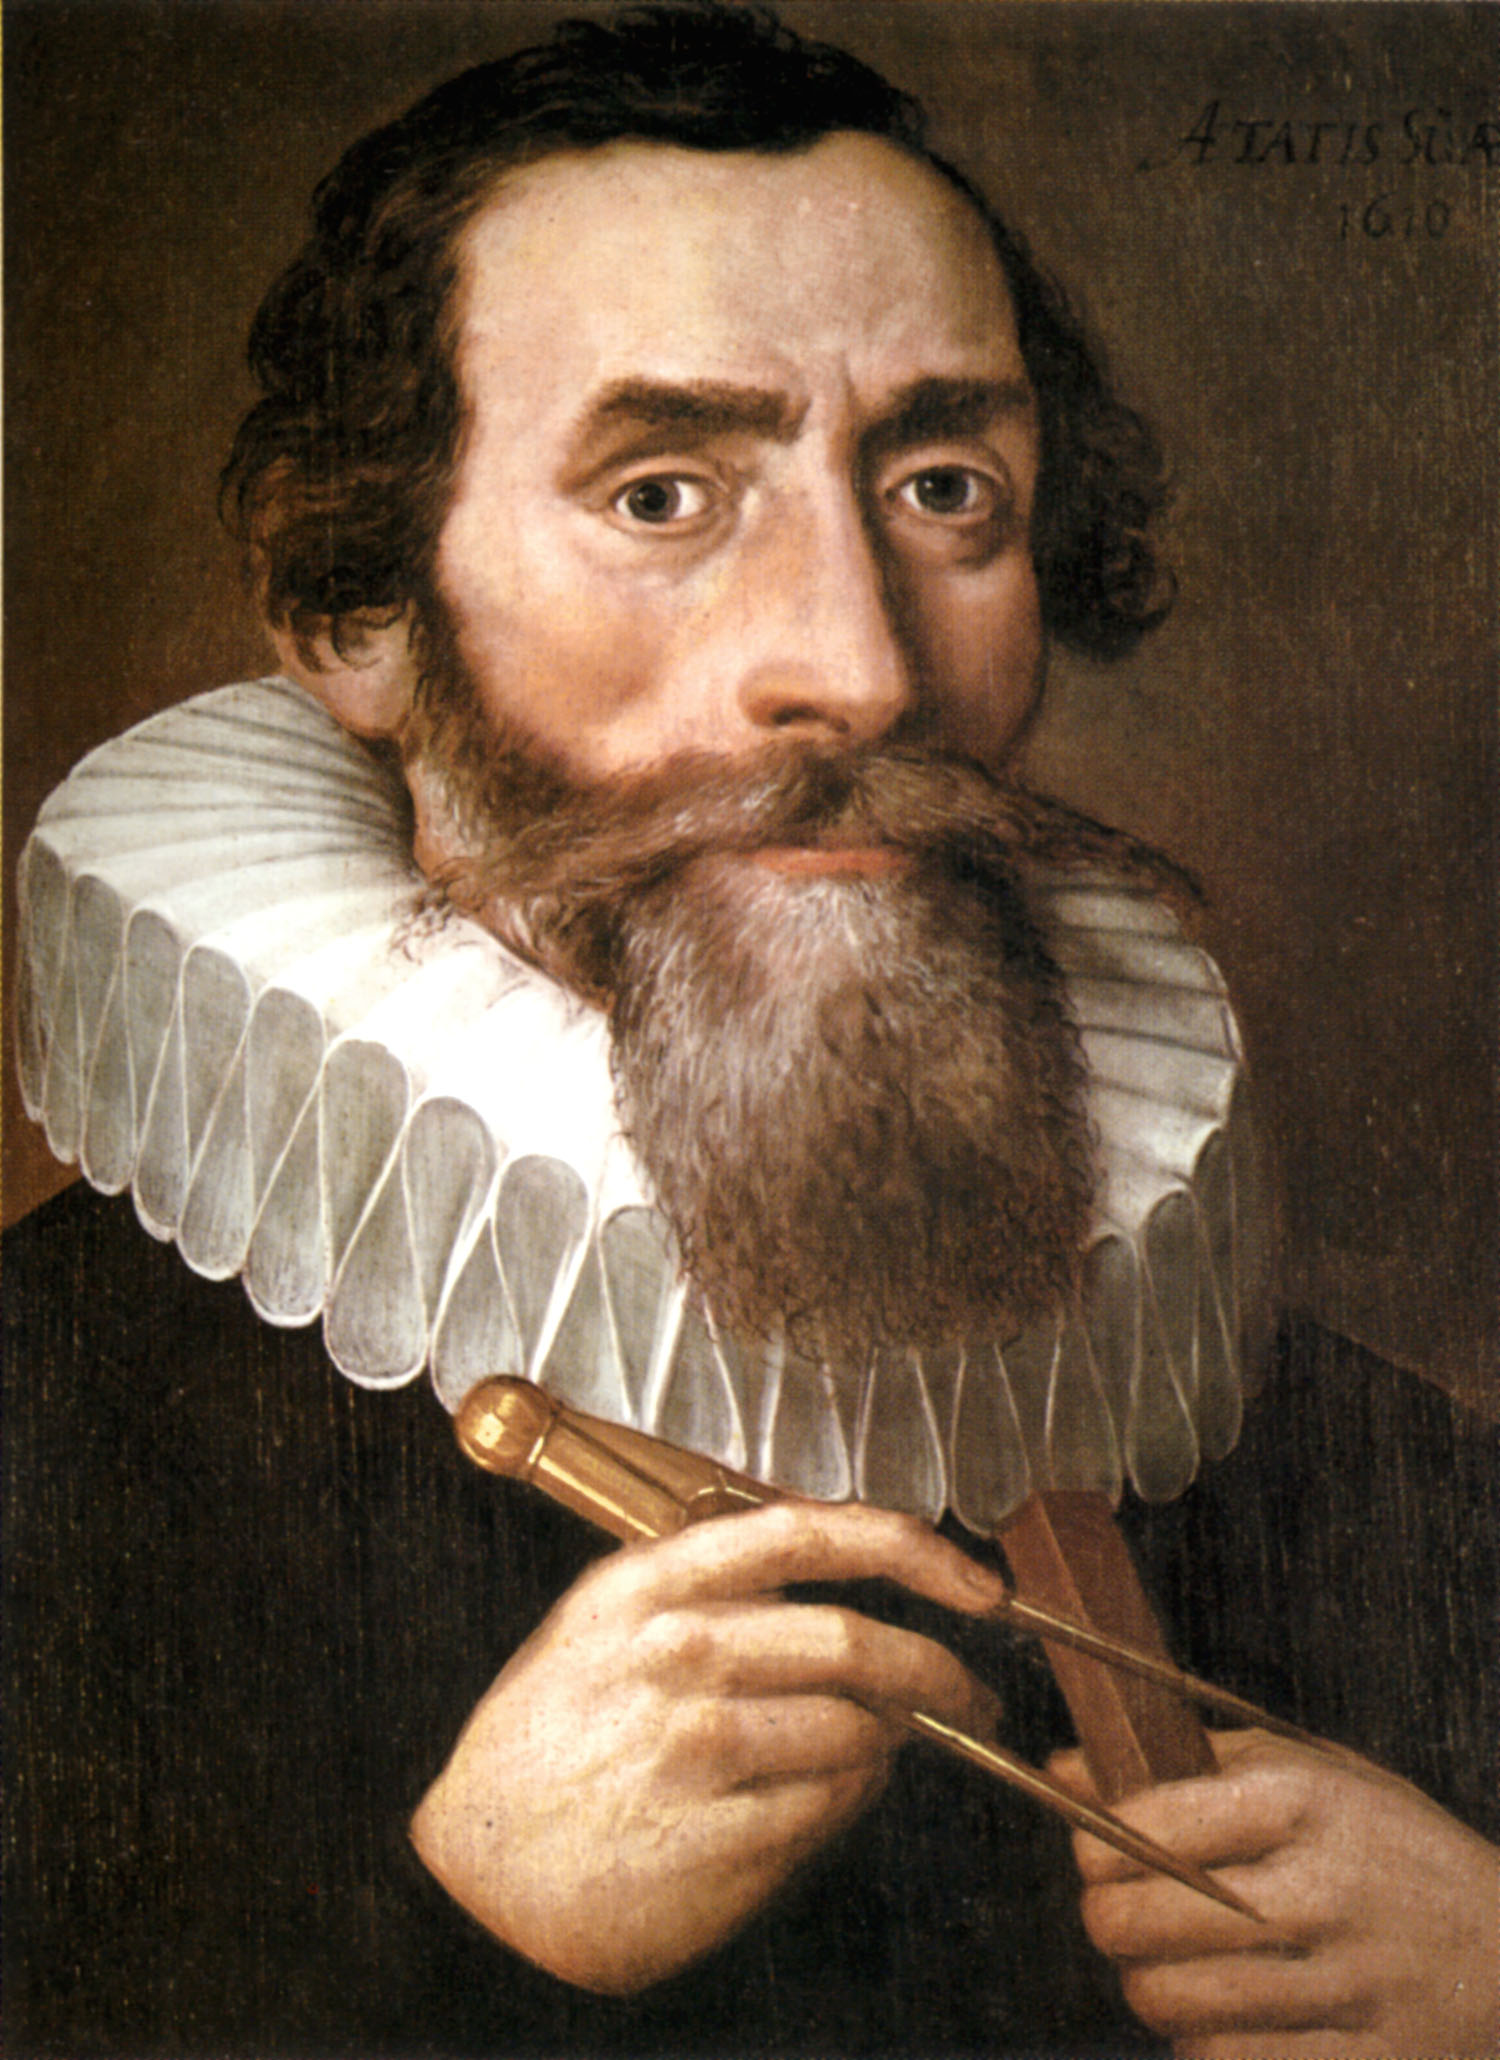
\includegraphics[width=0.3\textwidth]{kepler.jpg}
 \caption{Ein Bild von Kepler.\label{fig:beispiel}}
\end{figure}

In Tabellen ist darauf zu achten, dass möglichst wenig vertikale Striche verwendet werden, wie im Beispiel in \tab{tab:beispiel} gezeigt.
\begin{table}[h]
 \centering
 \caption{Bahntypen als Funktion der Exzentrizit\"at.\label{tab:beispiel}}
 \begin{tabular}{cl}
  \tb{Wert der Exzentrizit\"at} & \multicolumn{1}{c}{\tb{Bahntyp}} \\
  \hline
  \hline
  $\epsilon = 0$ & Kreis \\
  $0 < \epsilon < 1$ & Ellipse \\
  $\epsilon = 1$ & Parabel \\
  $\epsilon > 1$ & Hyperbel \\
  \hline
 \end{tabular}
\end{table}

\section{Referenzieren und Zitieren}

Das richtige Referenzieren und Zitieren ist Grundvoraussetzung für eine erfolgreiche Arbeit. Die TU Braunschweig setzt seit dem 15.07.2014 routinemäßig
die Plagiatserkennungssoftware \tb{docoloc} ein, um alle Arbeiten von Studenten auf Plagiarismus zu prüfen.

Es ist also mit äußerster Sorgfalt bei der Verwendung von Textstellen, Herleitungen, Bildern und Daten aus der Literatur
bzw. externen Quellen vorzugehen.

Für jede Wiedergabe aus der Literatur (z.B. Zitat) folgt die Referenz direkt im Anschluss (nicht erst am Ende des Satzes!). Eine Autor-Jahr-Notation ist 
empfohlen, welche mit folgendem Beispiel einfach in dieser Vorlage umgesetzt werden kann:
\begin{itemize}
 \item Ein Zitat mit Klammern: \citep{autor2012}
 \item Ein Zitat ohne Klammern: \cite{autor2012}
\end{itemize}

Literaturangaben werden durch \tb{bibtex} (Datei: \ts{literatur.bib}) übernommen und müssen enthalten:
\begin{itemize}
 \item Bei Artikeln aus Zeitschriften: Verfassernamen, Titel des Artikels, Name der Zeitschrift, Bandnummer, 
       Erscheinungsjahr, Nummer des Heftes, Anfangs- und Schlussseite des Artikels
 \item Bei Büchern: Verfassername, Buchtitel, Bandnummer, Auflage, Verlagsort, Verlag und Erscheinungsjahr     
 \item Bei Internet-Seiten: URL sowie Zugriffsdaten
 \item Informationen, die man etwa aus persönlichen Gesprächen erhalten hat, lassen sich ebenfalls eintragen, z.B.:
       \ts{Max Mustermann, persönliches Gespräch, Datum}
\end{itemize}

\section{Programmieren}

Basierend auf einer Top-Down-Analyse des vorgegebenen Problems können zunehmend verfeinerte 
Flussdiagramme erstellt werden, die bereits eine Programmstruktur implizieren und die Übersicht bei komplexen
Programmen erhöhen.

Programme sollten allgemein so geschrieben werden, daß ein Interessierter deren Funktion und deren Ablauf in 
groben Schritten ohne Dokumentation nachvollziehen kann (selbstdokumentierend). Hierzu dienen Kommentare im Quelltext,
eine optische Gliederung des Programmtextes und die weitestgehende Verwendung von strukturierter
Programmierung. Ein Anwender sollte vom Programm geleitet und über den Ablauf informiert werden. Benutzereingaben
sollten möglichst vom Programm auf Plausibilität gecheckt werden.

Im Folgenden ist ein Code-Beispiel (Fortran) gezeigt, welches die typischen Elemente jedes Haupt- und Unterprogramms zeigt, wobei Anmerkungen darin zwischen  
``$<<$'' und ``$>>$'' gefasst und damit nicht Teil des Quellcodes bzw. der Kommentare des Codes sind. Es handelt sich bei dem Kopfteil um eine Struktur,
die es ermöglicht, eine automatische Dokumentation mittels der Software \tb{Doxygen} zu erstellen:

\begin{verbatim}
!------------------------------------------------------------------------------
!
!> @anchor      initGravityPotential  << Doxygen-Kommentare beginnen in Fortran
!!                                    << mit !!, der erste jedoch mit !>. Ein 
!!                                    << @anchor stellt später einen Link auf  
!!                                    << diese Funktion zur Verfügung >>
!!
!! @brief       Initialization...     << Kurzbeschreibung der Funktion >>
!! @author      Max Mustermann        << Name des Autors >>
!!
!! @date        <ul>                  << @date erlaubt eine Revisionshistorie
!!                                    << zu führen >>
!!                <li> 02.10.2012 (initial design)    </li>
!!                <li> 31.05.2013 (code optimization) </li>
!!                <li> 19.08.2013 (added ...)         </li>
!!              </ul>
!!
!! @param[in]   cpath       Path to...       << Beschreibung der Inputgrößen
!! @param[in]   imodel      Model to be...
!! @param[out]  cout        Output string... << 'out' für Outputgrößen
!!
!! @details     This routine initializes the... << Detaillierte Funktions-
!!              ....                            << beschreibung, in die z.B. auch
!!                                              << auch die verwendeten Quellen
!!                                              << bzw. Literaturangaben gehören.
!!
!!-----------------------------------------------------------------------------
subroutine initGravityPotential(cpath,imodel,cout)

  implicit none              << In Fortran immer gut, damit keine Variablen
                             << implizit deklariert sind, z.B. wäre dann
                             << ein 'a' automatisch ein integer

                             
  << DEKLARATIONSTEIL>>
  
  
  !** interface              << Zuerst die Schnittstellenvariablen
  !------------------------------------------ 
  character(len=*), intent(in)  :: cpath
  integer,          intent(in)  :: imodel
  !------------------------------------------

  !** local                  << Dann die lokalen Variablen
  !---------------------------------------------------
  character(len=255)           :: cbuf      ! character buffer
  character(len=*), parameter  :: csubid = "initGravityPotential"
  ...
  
  integer :: i                    ! loop counter
  integer :: ich                  ! input channel
  integer :: ierr                 ! error flag
  ...
  
  real(dp)  :: fac                ! multiplication factor
  ...
  !--------------------------------------------------------
  
  << Nun beginnt der eigentliche PROGRAMMTEXT >>
    
  coeffInitialized = .false.    ! as a new initialization is started...

  !============================================================================
  !
  ! Decide on which model to use (default: EIGEN-GL04C)
  ! 
  !---------------------------------------------------------
  
  << Verwendung von logischen 'Blöcken', um Lesbarkeit zu erhöhen...>>
  
  !** check imodel validity
  if(imodel == EGM96 .or. imodel == EGM08) then
    nmodel = imodel  << Einrückung erhöhen die Lesbarkeit! >>
  else
    nmodel = EIGEN_GL04C
  end if

  !============================================================================
  !
  !   Read earth radius and...
  !
  !--------------------------------------------------------------------------

  flag_mu   = .false.
  flag_rekm = .false.

  do i = 1,imax

    read(ich,'(a)',iostat=ios) cbuf
      
    !** earth gravity constant
    if(index(cbuf, "earth_gravity_constant") /= 0) then

      read(cbuf,*) ctemp, mu
      ...
      
    end if
    
    ...
    
  end do
  
  ...

\end{verbatim}

Während die obige Darstellung bereits eine gute Möglichkeit darstellt, um Ausschnitte von Quellcode auch in der eigenen Arbeit zwecks Beschreibung 
wiederzugeben, gibt es auch weitere Pakete, die etwa auch Syntax-Highlighting unterstützen. Eines davon ist z.B. \tb{minted}.

%-----------------------------------
\subsection{Unterunterkapitel}
\label{cha:Unterunterkapitel}
%-----------------------------------
  \chapter{Ergebnisse}
\label{sec:ergebnisse}

\section{Grafiken und Text}

Im Ergebnis-Teil sollen die Ergebnisse vorgestellt werden, für das Beispiel einer Software-Entwicklung also die mit der entwickelten Software erzielbaren 
Ergebnisse. Im Falle einer Simulationsentwicklung könnte man hier verschiedene Simulationsszenarien definieren und unter verschiedenen Randbedingungen 
vorstellen.

Es ist dabei darauf zu achten, dass ein ausgewogenes Verhältnis von Bild und Text besteht. Alle in den Plots vorkommenden Linien sind zu erklären. Jeder Plot 
benötigt eine vollständige Achsenbeschriftung und ggf. eine Legende. Eine Grafik muss immer selbsterklärend sein, d.h. man muss mit Grafik und Bildunterschrift 
allein in der Lage sein, das Gezeigte zu verstehen.

Auch bei den Ergebnissen soll weiterhin auf den roten Faden geachtet werden. Der Leser soll Stärken und Schwächen des Tools / der Simulation / der Konstruktion 
kennenlernen.

Um Plots zu erstellen, lässt sich ebenfalls TikZ nutzen (wie auch für WBS, Zeitplan, etc.). Der Vorteil ist, dass alle Beschriftungen einer Grafik auch 
dieselbe Schrift und -größe tragen, wie auch der Haupttext. Darüber hinaus sind TikZ-Grafiken auch Vektorgrafiken, sodass Qualitätsverluste nicht zu erwarten 
sind, wie das etwa bei PNG oder JPG der Fall wäre.

Beispiel für das Plotten von zwei verschiedenen Kurven aus Datenfiles, welches das Paket \tb{pgfplots} nutzt (siehe auch sehr ausführliche Dokumentation mit 
zahlreichen Beispielen online!):

\begin{figure}[h!]
 \centering
 \begin{tikzpicture}
  \begin{axis}[
       xlabel = {Anzahl entfernter Objekte pro Mission},
       ylabel = {Missionskosten in USD/kg (FY14)},
       xlabel near ticks,
       ylabel near ticks,
       xmin   = 2,
       xmax   = 10,
       xtick  = {2,4,6,8,10},
       minor x tick num={1},
       minor y tick num={1},
       %ymin   = 0,
       %ymax   = 400000,
       scaled ticks = false,
       ymajorgrids,
       yminorgrids,
       xmajorgrids,
       xminorgrids,
       legend entries={$m_t=5.5\;t$, $m_t=1.4\;t$},
       legend style={at={(0.5,-0.2)}, anchor=north, draw=none},
       legend cell align = left
  ]
    \addplot[mark=square,   mark options=solid, solid]              	table {tikz/data/mtm-cost-per-kg-cp.dat};
    \addplot[mark=asterisk, mark options=solid, densely dashed]     	table {tikz/data/mtm-cost-per-kg-cp-low-mass.dat};    
  
  \end{axis}
\end{tikzpicture}
 \caption{Vergleich der Kosten pro kg entfernten Schrotts für hohe und mittlere Objektmassen.\label{abb:vergleich}}
\end{figure}

Auch das Plotten von Funktionen ist sehr einfach, wie \abb{abb:x2} für das simple Beispiel einer quadratischen Funktion zeigt.

\begin{figure}[h!]
  \centering
  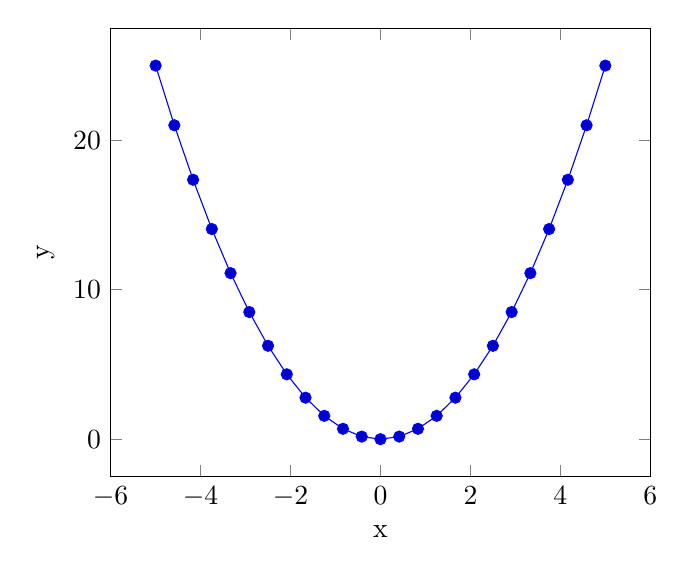
\begin{tikzpicture}
    \begin{axis}[
       xlabel = x,
       ylabel = y
    ]
    
      \addplot {x^2};
  
    \end{axis}
  \end{tikzpicture}
  \caption{Die Funktion $y=x^2$.\label{abb:x2}}
\end{figure}

Sollte nicht TikZ verwendet werden, ist auch \tb{Gnuplot} zu empfehlen. Allerdings ist dann darauf zu achten, dass sämtliche Beschriftungen gut lesbar sind und 
auch die Grafiken in der entsprechenden Auflösung, ohne Artefakte, etc. im Dokument erscheinen.

\section{Erstellen dieses Dokuments}

Um das vorliegende Dokument zu erstellen, muss die Datei \ts{vorlage.tex} mit \tb{pdflatex} kompiliert werden. Alle üblichen Entwicklungsumgebungen für Latex 
stellen diese Funktion zur Verfügung (z.B. Kile unter Linux, MikTeX unter Windows, oder TeXShop auf dem Mac).

Dazu wird die Dokumentenklasse \tb{tubsreprt} benötigt, welche das Corporate Design der TU Braunschweig umsetzt. Diese findet man, samt Installationsanleitung 
unter \url{http://www.enricojoerns.de/tubslatex/} (aktueller Release: 1.0.3).

Wichtig, damit auch das Symbol- und Abkürzungverzeichnis funktionieren, ist die Ausführung des Befehls \tb{makeglossaries} ebenfalls auf die Datei 
\ts{vorlage.tex} angewandt. Die Erstellung des Dokuments verläuft also in mehreren Schritten:
\begin{itemize}
 \item pdflatex auf \ts{vorlage.tex} (erzeugt die für makeglossaries benötigten Dateien!)
 \item makeglossaries auf \ts{vorlage.tex} (erstellt das Abkürzungs- und Symbolverzeichnis)
 \item pdflatex auf \ts{vorlage.tex} (ggf. mehrmals!) erstellt nun das Dokument mit allen Referenzen
\end{itemize}
Der Befehl makeglossaries muss in der Regel manuell in der Entwicklungsumgebung eingestellt werden, was für die verschiedenen Typen unterschiedlich ist. Daher 
am besten Google befragen (z.B. ``Kile makeglossaries'').
  \chapter{Zusammenfassung}

In der Zusammenfassung (mindestens 1,5 Seiten) sollen die theoretische Herleitung
und die wesentlichen Ergebnisse so aufgelistet werden, dass sie ohne Kenntnis der
vorherigen Abhandlung verständlich sind. Dabei wird in der Vergangenheit geschrieben und die wichtigsten Ergebnisse
der Arbeit wiedergegeben.
  \chapter{Fazit und Ausblick}

Ein kurzer Ausblick (max. ca. 1 Seite) kann dazu dienen, bei
Bearbeitung der gestellten Aufgabe entstandene neue Fragestellungen für zukünftige
Untersuchungen zu nennen.

  %===================================================
  %
  % Literaturverzeichnis
  %
  %---------------------------------------------------
  \addcontentsline{toc}{chapter}{Literaturverzeichnis}
    \bibliographystyle{elsarticle-harv}
    \bibliography{literatur}
  
  %===================================================
  %
  % Abbildungsverzeichnis
  %
  %---------------------------------------------------
  \addcontentsline{toc}{chapter}{Abbildungsverzeichnis}
  \listoffigures
  \newpage
  
  %===================================================
  %
  % Tabellenverzeichnis
  %
  %---------------------------------------------------
  \addcontentsline{toc}{chapter}{Tabellenverzeichnis}
  \listoftables							% Tabellenverzeichnis
  \newpage
  
  %===================================================
  %
  % Symbol- und Abkürzungsverzeichnis
  %
  %---------------------------------------------------
  \chapter*{Symbolverzeichnis}						% Symbolverzeichnis
    \addcontentsline{toc}{chapter}{Symbolverzeichnis}			% fügt Symbolverzeichnis trotz * in das Inhaltsverzeichnis ein
          \printglossary[type=symbolslist, title=Symbole und Indizes]		% symbols
    \printglossary[type=acronymlist, title=Abk\"urzungen]		% abbreviations
 \glsaddall 
  %===================================================
  %
  % Anhang
  %
  %---------------------------------
  \begin{appendix}
    \chapter{Projektmanagement}
\label{cha:projekt}

\section{Work Breakdown Structure}
\label{sec:wbs}

\begin{landscape}
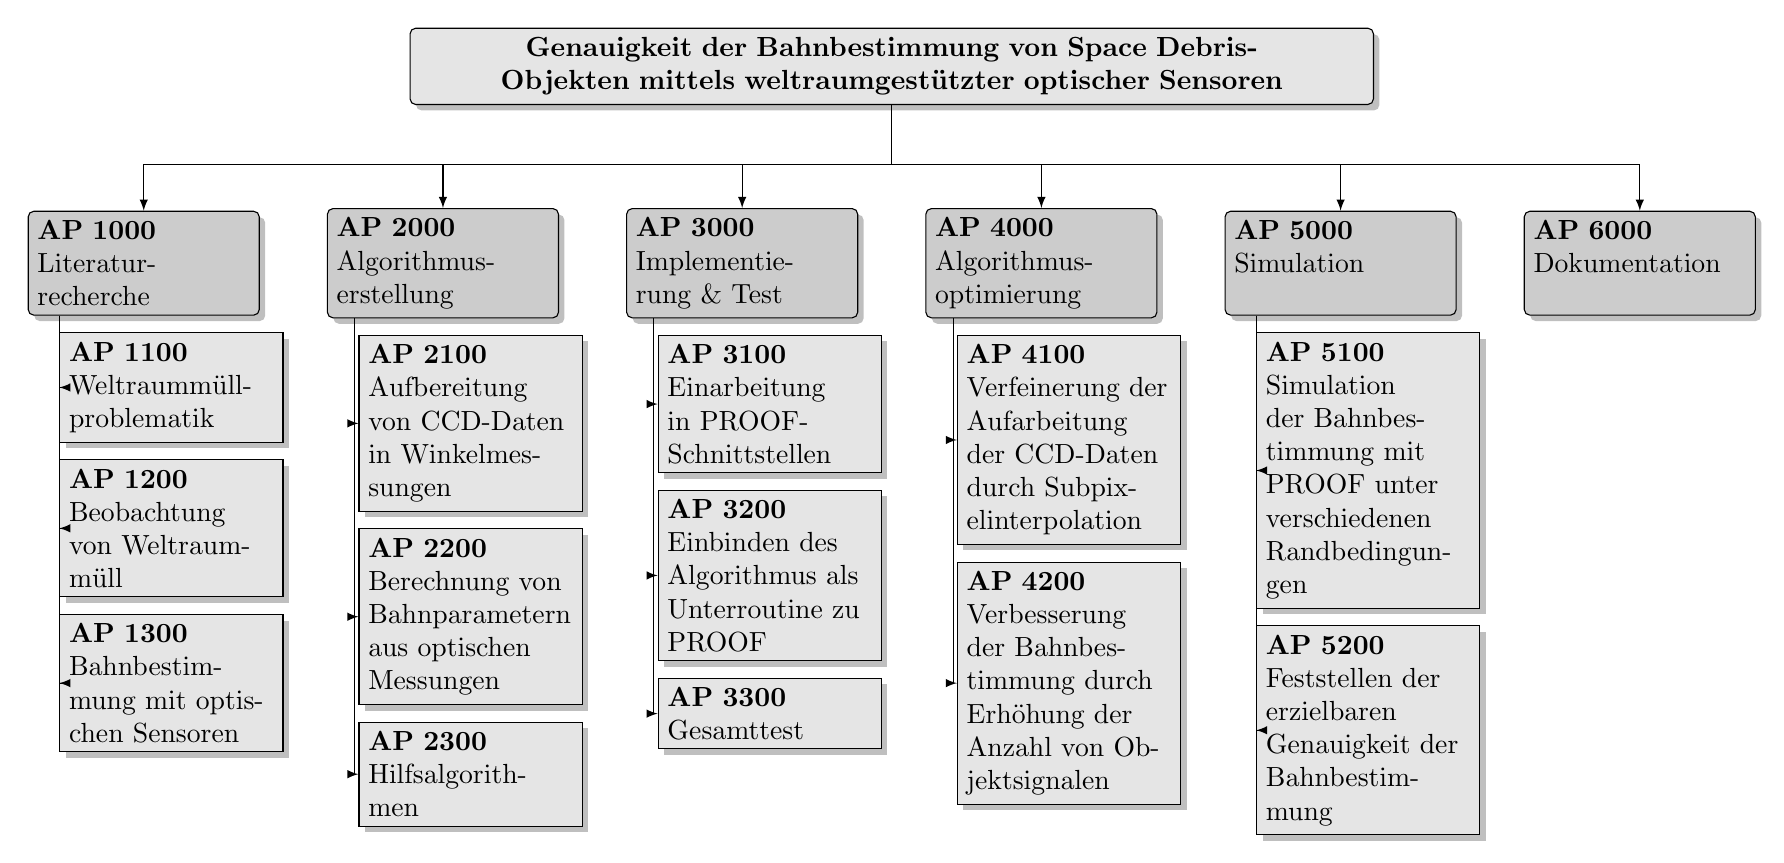
\begin{tikzpicture}[
  basic/.style   = {draw, text width=2.7cm, align=left, drop shadow, rectangle},
  root/.style    = {basic, text width=12cm, rounded corners=2pt, thin, align=center, fill=gray90},
  level 2/.style = {basic, rounded corners=2pt, thin, fill=gray80},
  level 3/.style = {basic, thin, fill=gray90, text width=2.6cm},
  level 1/.style={sibling distance=38mm}, edge from parent fork down, 
  edge from parent/.style={->,draw}, level distance=2.5cm,  >=latex]

% root of the the initial tree, level 1
\node[root] {\tb{Genauigkeit der Bahnbestimmung von Space Debris-Objekten mittels weltraumgest\"utzter optischer Sensoren}}
% The first level, as children of the initial tree
  child {node[level 2] (c1) {\tb{AP~1000} \\ Literatur-recherche}}
  child {node[level 2] (c2) {\tb{AP~2000} \\ Algorithmus-erstellung}}
  child {node[level 2] (c3) {\tb{AP~3000} \\ Implementie-rung \& Test}}
  child {node[level 2] (c4) {\tb{AP~4000} \\ Algorithmus-optimierung}}
  child {node[level 2] (c5) {\tb{AP~5000} \\ Simulation \\ $~~$}}
  child {node[level 2] (c6) {\tb{AP~6000} \\ Dokumentation \\ $~~$}};

% The second level, relatively positioned nodes
\begin{scope}[every node/.style={level 3}, node distance=6pt]
\node [below=of c1, xshift=10pt] (c11) {\tb{AP~1100} \\ Weltraumm\"ull-problematik};
\node [below=of c11] (c12) {\tb{AP~1200} \\ Beobachtung von Weltraum-m\"ull};
\node [below=of c12] (c13) {\tb{AP~1300} \\ Bahnbestim-mung mit optischen Sensoren};

\node [below=of c2, xshift=10pt] (c21) {\tb{AP~2100} \\ Aufbereitung von CCD-Daten in Winkelmessungen};
\node [below=of c21] (c22) {\tb{AP~2200} \\ Berechnung von Bahnparametern aus optischen Messungen};
\node [below=of c22] (c23) {\tb{AP~2300} \\ Hilfsalgorith-men};

\node [below=of c3, xshift=10pt] (c31) {\tb{AP~3100} \\ Einarbeitung in PROOF-Schnittstellen};
\node [below=of c31] (c32) {\tb{AP~3200} \\ Einbinden des Algorithmus als Unterroutine zu PROOF};
\node [below=of c32] (c33) {\tb{AP~3300} \\ Gesamttest};

\node [below=of c4, xshift=10pt] (c41) {\tb{AP~4100} \\ Verfeinerung der Aufarbeitung der CCD-Daten durch Subpixelinterpolation};
\node [below=of c41] (c42) {\tb{AP~4200} \\ Verbesserung der Bahnbestimmung durch Erh\"ohung der Anzahl von Objektsignalen};

\node [below=of c5, xshift=10pt] (c51) {\tb{AP~5100} \\ Simulation der Bahnbestimmung mit PROOF unter verschiedenen Randbedingungen};
\node [below=of c51] (c52) {\tb{AP~5200} \\ Feststellen der erzielbaren Genauigkeit der Bahnbestimmung};

\end{scope}

% lines from each level 1 node to every one of its "children"
\foreach \value in {1,2,3}
  \draw[->] (c1.212) |- (c1\value.west);

\foreach \value in {1,2,3}
  \draw[->] (c2.212) |- (c2\value.west);

\foreach \value in {1,2,3}
  \draw[->] (c3.212) |- (c3\value.west);

\foreach \value in {1,2}
  \draw[->] (c4.212) |- (c4\value.west);

\foreach \value in {1,2}
  \draw[->] (c5.212) |- (c5\value.west);
  
\end{tikzpicture}
\end{landscape}

\section{Zeitplan}
\label{sec:zeitplan}

\begin{landscape}
%\noindent\resizebox{\textwidth}{!}{	% Einfügen, falls zu groß
\begin{ganttchart}[hgrid,
                   time slot format = isodate, 
                   x unit=0.28cm,	% Zum komprimieren des Charts in x-Richtung
                   %y unit chart=0.7cm,
                   %compress calendar,	% Komprimiert den Chart in der Breite
                   calendar week text = {Woche~\currentweek},
                   chart element start border = right,
                   bar/.append style={fill=blue!40, rounded corners=2pt},
                   bar incomplete/.append style={fill=blue!10},
                   bar label node/.append style={align=left, text width=7cm},
                   group label node/.append style={align=left, text width=8cm},
                   milestone label node/.append style={align=left, text width=8cm},
                   bar progress label node/.style={right=2mm},
                   progress label text = {\pgfmathprintnumber[precision=0, verbatim]{#1}\%},
                  ]{2013-01-01}{2013-02-23}
  \gantttitlecalendar{year, month=shortname, week}\\
  %\gantttitle{2013}{59}\\
  \ganttgroup{AP 1000: Literaturrecherche}{2013-01-01}{2013-02-01}\\
  \ganttbar[progress=50]  {AP 1100: Weltraummüllproblematik}{2013-01-01}{2013-01-08}\\
  \ganttlinkedbar {AP 1200: Beobachtung von Weltraummüll}{2013-01-09}{2013-01-17}\\
  \ganttlinkedbar {AP 1300: Bahnbestimmung mit optischen Sensoren}{2013-01-17}{2013-02-01}\\
  %\ganttbar[progress=100]{AP 1300: TEXT}{2013-01-01}{2013-01-30}\\	% Beispiel für Fortschrittsbalken!
  
  \ganttgroup{AP 2000: Algorithmuserstellung}{2013-02-02}{2013-02-23}\\
  \ganttbar  {AP 2100: ...}{2013-02-02}{2013-02-09}\\
  \ganttbar  {AP 2200: ...}{2013-02-10}{2013-02-19}\\
  
  \ganttmilestone{Meilenstein}{2013-02-20}\\
  
 \end{ganttchart}
%}
\end{landscape}

\section{Work Package Description}
\label{sec:wpd}

\begin{table}[!h]
 \begin{center}
  \begin{tabular}{|p{35mm}||p{55mm}|p{50mm}||p{40mm}|}
   \hline
   \multicolumn{3}{|l||}{\textbf{}} & \multicolumn{1}{c|}{}\\
   \multicolumn{3}{|l||}{\textbf{}} & \multicolumn{1}{c|}{\textbf{AP 1100}}\\
   \multicolumn{3}{|l||}{\textbf{}} & \multicolumn{1}{c|}{}\\
   \hline\hline
   \textbf{Titel} & \multicolumn{2}{p{7cm}||}{\textbf{Genauigkeit der Bahnbestimmung von Space Debris-Objekten mittels weltraumgestützter optischer Sensoren}} 
& \textbf{Seite:} 1 von 1\\
   \hline
   \textbf{Verantwortlicher} & \multicolumn{2}{l||}{Sebastian Stabroth} & \textbf{Version:} 1.0\\
   \hline
   \multicolumn{3}{|l||}{} & \textbf{Datum:} 25.06.2003\\
   \hline\hline
   \textbf{Beginn} & \multicolumn{2}{l||}{T$_0$} & \\
   \hline
   \textbf{Ende} & \multicolumn{2}{l||}{T$_0$+1 Woche} & \textbf{Dauer}: 1 Woche\\
   \hline\hline
   \textbf{Bearbeiter} & \multicolumn{3}{l|}{Sebastian Stabroth}\\
   \hline\hline
   \multicolumn{4}{|p{150mm}|}{\textbf{Ziele:}}\\
   \multicolumn{4}{|p{150mm}|}{$\bullet$ Kenntnis über die Weltraummüllumgebung, Bahnbereiche von Space Debris-Populationen, Objektanzahlen und -größen}\\
   \multicolumn{4}{|p{150mm}|}{}\\
   \multicolumn{4}{|p{150mm}|}{\textbf{Input:}}\\
   \multicolumn{4}{|p{150mm}|}{$\bullet$ Literatur zum Thema Weltraummüll}\\
   \multicolumn{4}{|p{150mm}|}{}\\
   \multicolumn{4}{|p{150mm}|}{\textbf{Schnittstellen zu anderen APs:}}\\
   \multicolumn{4}{|p{150mm}|}{$\bullet$ \textbf{AP~5100} zur Simulation der Bahnbestimmung von Weltraummüll}\\
   \multicolumn{4}{|p{150mm}|}{}\\
   \multicolumn{4}{|p{150mm}|}{\textbf{Aufgaben:}}\\
   \multicolumn{4}{|p{150mm}|}{$\bullet$ Einlesen in die Thematik Weltraummüll}\\
   \multicolumn{4}{|p{150mm}|}{}\\
   \multicolumn{4}{|p{150mm}|}{\textbf{Ergebnisse:}}\\
   \multicolumn{4}{|p{150mm}|}{$\bullet$ Verständnis der Weltraummüllproblematik}\\
   \hline
  \end{tabular}
 \end{center}
\end{table}

\clearpage

\begin{table}[!h]
 \begin{center}
  \begin{tabular}{|p{35mm}||p{55mm}|p{50mm}||p{40mm}|}
   \hline
   \multicolumn{3}{|l||}{\textbf{}} & \multicolumn{1}{c|}{}\\
   \multicolumn{3}{|l||}{\textbf{}} & \multicolumn{1}{c|}{\textbf{AP 1200}}\\
   \multicolumn{3}{|l||}{\textbf{}} & \multicolumn{1}{c|}{}\\
   \hline\hline
   \textbf{Titel} & \multicolumn{2}{p{7cm}||}{\textbf{Titel des Arbeitspakets}} & \textbf{Seite:} X von Y\\
   \hline
   \textbf{Verantwortlicher} & \multicolumn{2}{l||}{Dein Name} & \textbf{Version:} 1.1\\
   \hline
   \multicolumn{3}{|l||}{} & \textbf{Datum:} DD.MM.YYYY\\
   \hline\hline
   \textbf{Beginn} & \multicolumn{2}{l||}{T$_0$} & \\
   \hline
   \textbf{Ende} & \multicolumn{2}{l||}{T$_0$+X Wochen} & \textbf{Dauer}: X Wochen\\
   \hline\hline
   \textbf{Bearbeiter} & \multicolumn{3}{l|}{Dein Name}\\
   \hline\hline
   \multicolumn{4}{|p{150mm}|}{\textbf{Ziele:}}\\
   \multicolumn{4}{|p{150mm}|}{$\bullet$ Ziel 1}\\
   \multicolumn{4}{|p{150mm}|}{$\bullet$ Ziel 2}\\
   \multicolumn{4}{|p{150mm}|}{$\bullet$ ...}\\
   \multicolumn{4}{|p{150mm}|}{}\\
   \multicolumn{4}{|p{150mm}|}{\textbf{Input:}}\\
   \multicolumn{4}{|p{150mm}|}{$\bullet$ Input 1}\\
   \multicolumn{4}{|p{150mm}|}{$\bullet$ ...}\\
   \multicolumn{4}{|p{150mm}|}{}\\
   \multicolumn{4}{|p{150mm}|}{\textbf{Schnittstellen zu anderen APs:}}\\
   \multicolumn{4}{|p{150mm}|}{$\bullet$ \textbf{AP XXXX} Beschreibung}\\
   \multicolumn{4}{|p{150mm}|}{$\bullet$ \textbf{AP ....} ...}\\
   \multicolumn{4}{|p{150mm}|}{}\\
   \multicolumn{4}{|p{150mm}|}{\textbf{Aufgaben:}}\\
   \multicolumn{4}{|p{150mm}|}{$\bullet$ Aufgabe 1}\\
   \multicolumn{4}{|p{150mm}|}{$\bullet$ ...}\\
   \multicolumn{4}{|p{150mm}|}{}\\
   \multicolumn{4}{|p{150mm}|}{\textbf{Ergebnisse:}}\\
   \multicolumn{4}{|p{150mm}|}{$\bullet$ Ergebnis 1}\\
   \multicolumn{4}{|p{150mm}|}{$\bullet$ ...}\\
   \hline
  \end{tabular}
 \end{center}
\end{table}
    %\include{WEITERER ANHANG}
  \end{appendix}

\end{document}
